\documentclass[10pt,a4paper]{article}
\usepackage[margin=.5in,bottom=1in]{geometry}
\usepackage[utf8]{inputenc}
\usepackage[IL2]{fontenc}
\usepackage[czech]{babel}
\usepackage{microtype}
\usepackage{amssymb}
\usepackage{amsthm}
\usepackage{amsmath}
\usepackage{xcolor}
\usepackage{graphicx}

\usepackage[inline]{enumitem}

\theoremstyle{definition}
\newtheorem*{uloha}{Úloha}
\newtheorem*{bonus}{Nepovinný bonus}

\pagestyle{empty}

\newenvironment{res}{\proof}{\endproof}

\begin{document}

\renewcommand*{\proofname}{Řešení}

\section*{Řešení úloh s nálevkou}

\begin{uloha}
Nálevka má tvar rovnostranného kužele. Vypočítejte obsah plochy smáčené vodou v případě, že do nálevky nalijete 3 litry vody.
\end{uloha}

\begin{res}
Vlastně máme kužel, jehož objem je 3 litry a řezem je rovnostranný trojúhelník.
\[ 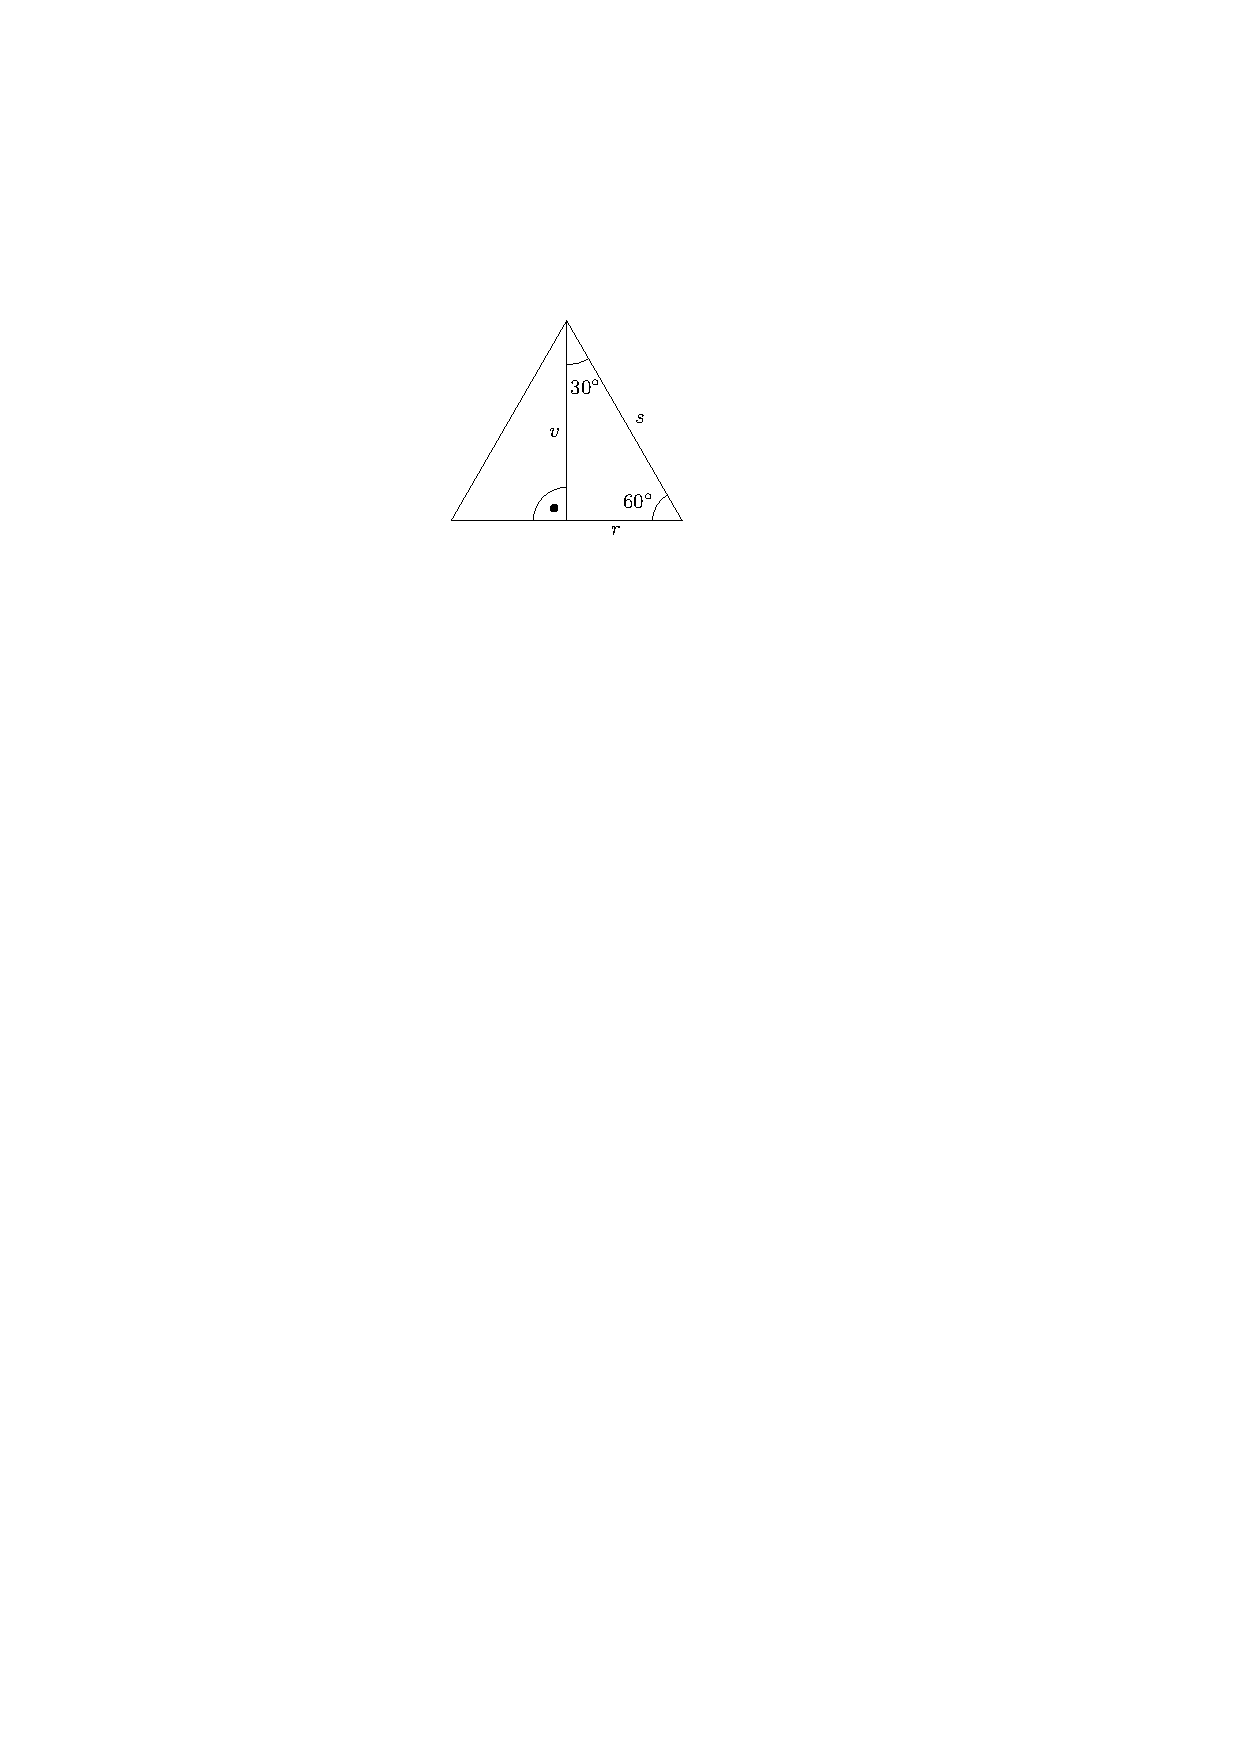
\includegraphics{trojuhelnik.pdf} \]
Buď pomocí goniometrických funkcí, nebo tak, že si to už pamatujeme, si vyjádříme (např.)
\[ r = \frac{\sqrt3}3 v, \]
což dosadíme do vzorce pro objem kužele
\[ V = \frac13 \pi r^2 v \]
a dostaneme
\[ 3 = V = \frac13 \pi \left(\frac{\sqrt3}3 v\right)^2 v = \frac13 \pi \frac39 v^2 v = \frac19 \pi v^3, \]
tedy
\[ v^3 = \frac{27}{\pi} \]
čili
\[ v = \sqrt[3]{\frac{27}{\pi}} = \frac{3}{\sqrt[3]{\pi}}. \]
Odtud dostáváme
\[ r = \frac{\sqrt3}3 v = \frac{\sqrt3}{\sqrt[3]{\pi}} \qquad \text a \qquad s = 2r = \frac{2\sqrt3}{\sqrt[3]{\pi}}. \]
Hledaný smáčený povrch (který nezahrnuje podstavu) se dopočte jako
\[ S = \pi r s = \pi \cdot \frac{\sqrt3}{\sqrt[3]{\pi}} \cdot \frac{2\sqrt3}{\sqrt[3]{\pi}} = 6 \sqrt[3]{\pi}. \]
\end{res}


\end{document}